% Die Arbeit besteht aus Kapiteln (chapter)
\chapter{Conceptual Design}

\section{General Design}
The goal of this thesis is to develop a system that allows generating large sets of images that are to be used for training neural networks. As this environment shall be used as a drop-in replacement for conventional methods such as taking photos and labeling those by hand, this implicates that the generated images must be of excellent quality and labeled.\\
At its core the system features at least one virtual environment (a "scene") and a robot. it allows users to operate in one of two modes: \textit{"manual control"} lets users take control of a virtual robot and maneuver it in the virtual scene. This includes accelerating, decelerating and steering the robot as well as resetting it in case of being unable to maneuver (this may be the case when the robot is flipped or trapped between objects). This mode can be used to evaluate the usefulness (e.g. mobility) of certain robot-bodies in certain environments.\\
The second mode of operation, \textit{"automatic scene recording"}, allows users to let the robot travel along preconfigured paths, let the system alter the scene and take screenshots from the robot's perspective in fixed intervals. This mode is used to create the sets of images.\\
Figure \ref{fig:use-cases} shows the high-level use-cases described in both modes.

\begin{center}
\noindent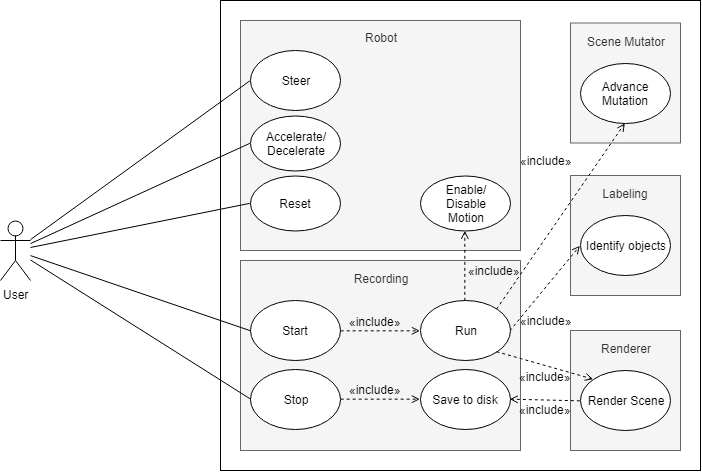
\includegraphics[width=15cm]{tex/img/ch04/Use_Cases_02.png}
\captionof{figure}{High level use cases}
\label{fig:use-cases}
\end{center}

\section{Frontend: Game Engine}

\subsection{TBD}

\subsubsection{TBD}
 
\paragraph{TBD} TBD
\paragraph{lelelel}

\section{Backend: Renderer}